\documentclass[../homework.tex]{subfiles}
 \graphicspath{{\subfix{../images/}}}

\begin{document}

\section{Методика решения}


\subsection{Осваиваем формулы}

Пример встроенной в строку формулы $a x^2 + b x + c = f(x)$.
Пишется так:

{\small
\begin{verbatim}
    Пример встроенной в строку формулы $a x^2 + b x + c = f(x)$.
\end{verbatim}
}

Центрированная формула без номера пишется так:
{\small
\begin{verbatim}
\[
d_{в} =
d_{*} \sqrt{\nu_{в}} =
53.1 \cdot 10^{-2} \cdot \sqrt{8.2} = 1.532 \text{ м}.
\]
\end{verbatim}
}
А отображается так:
%
\[
d_{в} =
d_{*} \sqrt{\nu_{в}} =
53.1 \cdot 10^{-2} \cdot \sqrt{8.2} = 1.532 \text{ м}.
\]
% Обратите внимание на закомментированную пустую строку (нужна, чтобы не было слишком большого интервала перед формулой), либо просто не оставляйте пустую строку перед центрированной формулой

Тоже формула без номера:
{\small
\begin{verbatim}
\begin{equation*}
    x_{*} =
    \cfrac{D_{к} - d_{*}}{2 \tan \alpha} =
    \cfrac{1.9 d_{*} - d_{*}}{2 \tan \alpha} =
    \cfrac{0.9 \cdot 53.1 \cdot 10^{-2}}{2} =
    0.248 \text{ м}.
\end{equation*}
\end{verbatim}
}
%
\begin{equation*}
    x_{*} =
    \cfrac{D_{к} - d_{*}}{2 \tan \alpha} =
    \cfrac{1.9 d_{*} - d_{*}}{2 \tan \alpha} =
    \cfrac{0.9 \cdot 53.1 \cdot 10^{-2}}{2} =
    0.248 \text{ м}.
\end{equation*}

\textbf{
    Не забывайте, что формулы~--- это обычные члены предложения, поэтому на них распространяются все известные вам правила пунктуации.
}

Формула с номером и \textit{меткой (label)} для ссылки на неё:\\
записывается так:
{\small
\begin{verbatim}
\begin{equation}
d(x) = \begin{cases}
        D_к - (D_к - d_*) \cfrac{x}{x_*}, & 0 < x \leq x_*, \\
        d_* + (d_в - d_*) \cfrac{x - x_*}{x_в - x_*}, & x > x_*.
\end{cases}
\label{eq:diameter}
\end{equation}
\end{verbatim}
}
а отображается так:
%
\begin{equation}
d(x) =
    \begin{cases}
        D_к - (D_к - d_*) \cfrac{x}{x_*}, & 0 < x \leq x_*, \\
        d_* + (d_в - d_*) \cfrac{x - x_*}{x_в - x_*}, & x > x_*.
    \end{cases}
\label{eq:diameter}
\end{equation}

Сослаться на уравнение можно с помощью команды \texttt{\\ref}.
Например, строка в tex-файле
{\small
\begin{verbatim}
    В уравнении (\ref{eq:diameter}) происходят странности...
\end{verbatim}
}
отобразится в <<В уравнении (\ref{eq:diameter}) происходят странности...>>.
То есть ссылаемся с помощью всё той же команды \texttt{ref}.


\subsection{Осваиваем рисунки}

Рассмотрим только вставку нумерованного и именованного рисунка, поскольку другие случаи в технических отчётах редки.

Чтобы вставить рисунок с подписью нужно сделать следующее:
{\small
\begin{verbatim}
\begin{figure}[h]
    \centering
    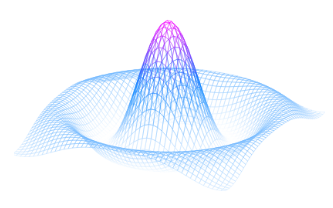
\includegraphics[width=0.4\textwidth]{fig_example.png}
    % Подпись
    \caption{Некоторый график}
    % Метка для ссылки на рисунок
    \label{fig:some_plot}
\end{figure}
\end{verbatim}
}
%
\begin{figure}[h]
    \centering
    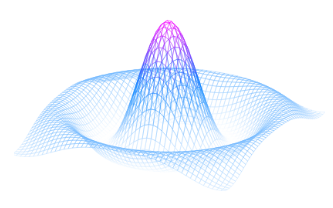
\includegraphics[width=0.4\textwidth]{fig_example.png}
    % Подпись
    \caption{Некоторый график}
    % Метка для ссылки на рисунок
    \label{fig:some_plot}
\end{figure}

Здесь важно помнить, что в преамбуле у нас есть фраза
{\small
\begin{verbatim}
\graphicspath{{\subfix{../images/}}}
\end{verbatim}
}
задающая папку, в которой хранятся картинки.
Поэтому мы можем указывать в \texttt{includegraphics} только имя файла.

Сослаться всё так же просто.
Вот пример:
{\small
\begin{verbatim}
На рисунке~\ref{fig:some_plot} изображена функция ,,сомбреро''.
\end{verbatim}
}
Отображается как: <<На рисунке~\ref{fig:some_plot} изображена функция ,,сомбреро''.>>

\textbf{
    Помните о том, что перекрёстные ссылки требуют двух компиляций.
}

\textbf{
    И не забывайте про неразрывные пробелы.
    Номера рисунков, таблиц и формул не должны стоять в начале строки без упоминания перед ними, что именно означает цифра.
}

Пример вставки двух рисунков в одной строке с разными подписями:

\figspace
\noindent
\begin{minipage}[t]{.5\textwidth}
    \centering
    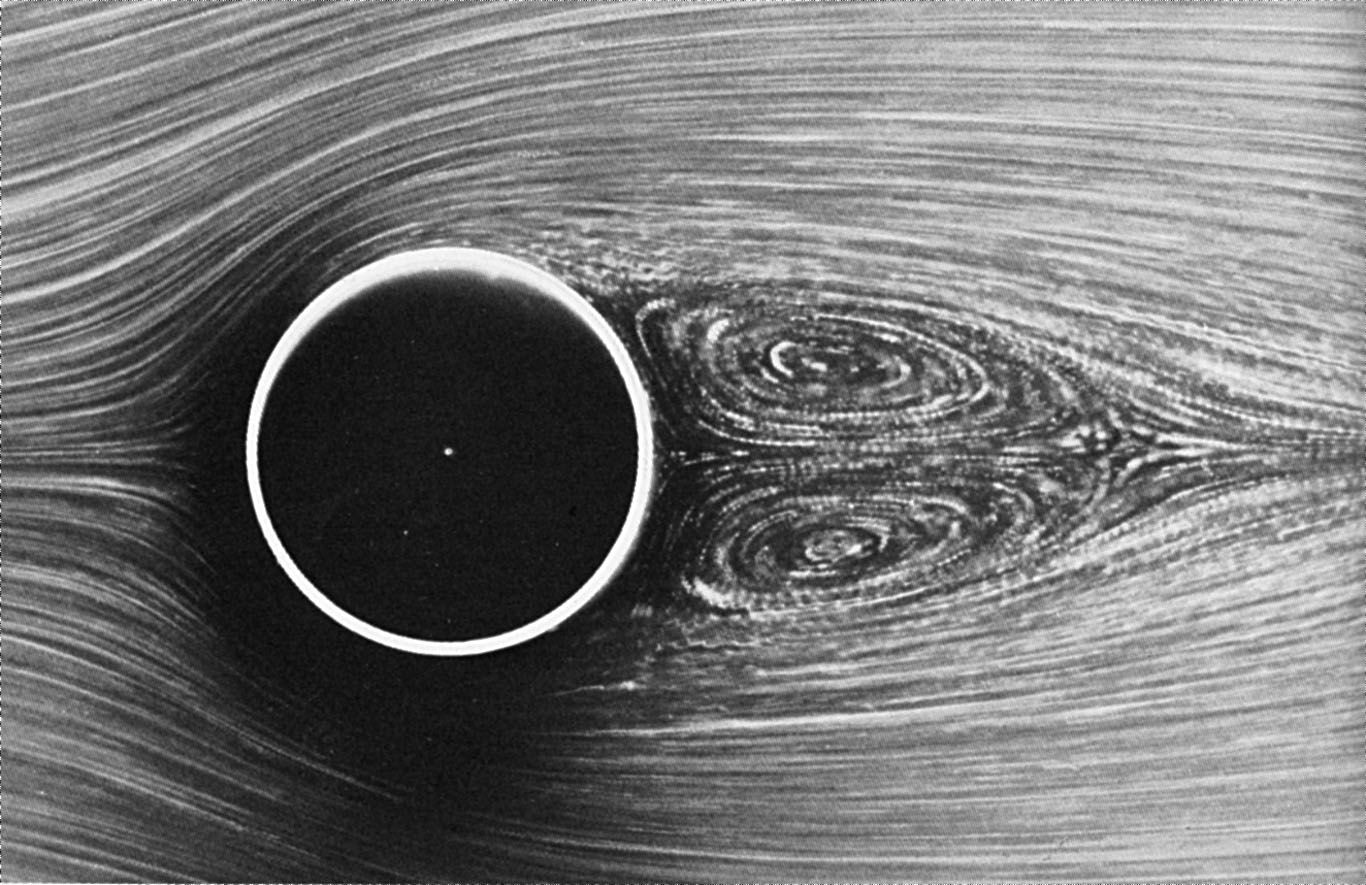
\includegraphics[width=0.95\linewidth]{gd_cylinder.png}
    \captionof{figure}{Обтекание цилиндра}
    \label{fig:cylinder}
\end{minipage}
%
\begin{minipage}[t]{.5\textwidth}
    \centering
    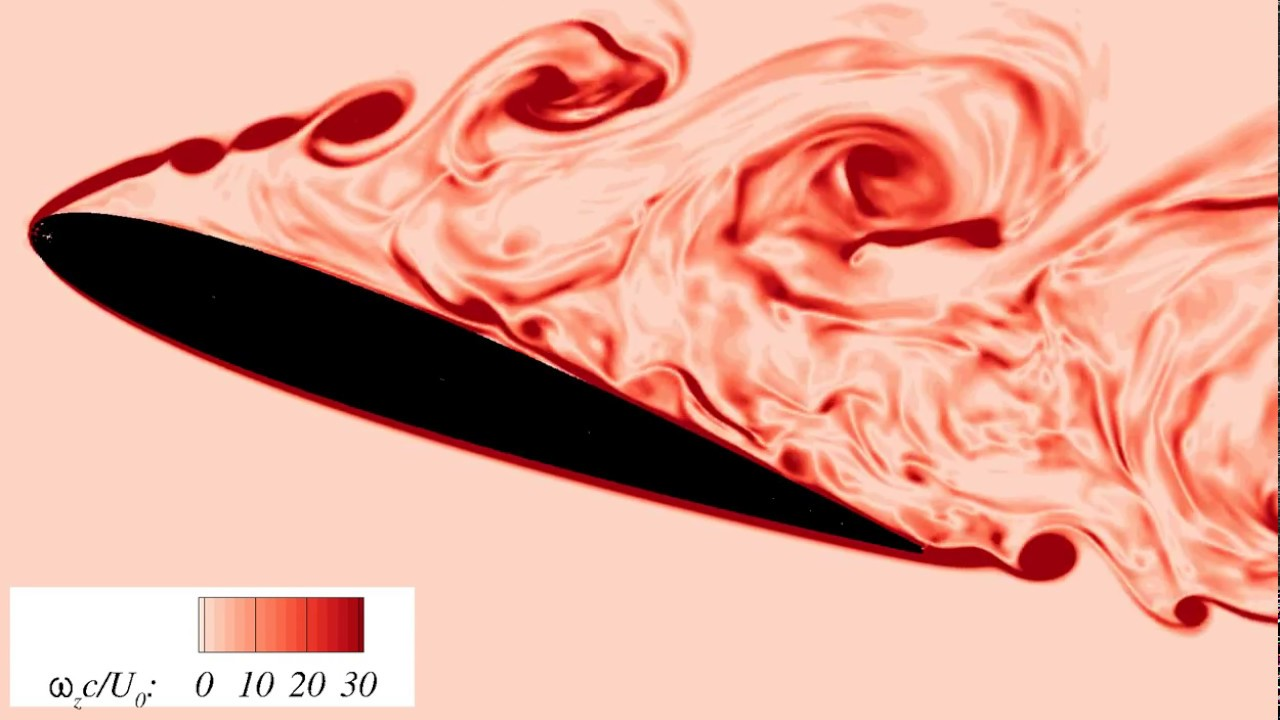
\includegraphics[width=0.95\linewidth]{airfoil.png}
    \captionof{figure}{Обтекание профиля крыла}
    \label{fig:airfoil}
\end{minipage}
\figspace

В исходнике рисунки~\ref{fig:a_cylinder} и~\ref{fig:airfoil} выглядят так:

{\small
\begin{verbatim}
Пример вставки двух рисунков в одной строке с разными подписями:

\noindent
\begin{minipage}[t]{.5\textwidth}
    \centering
    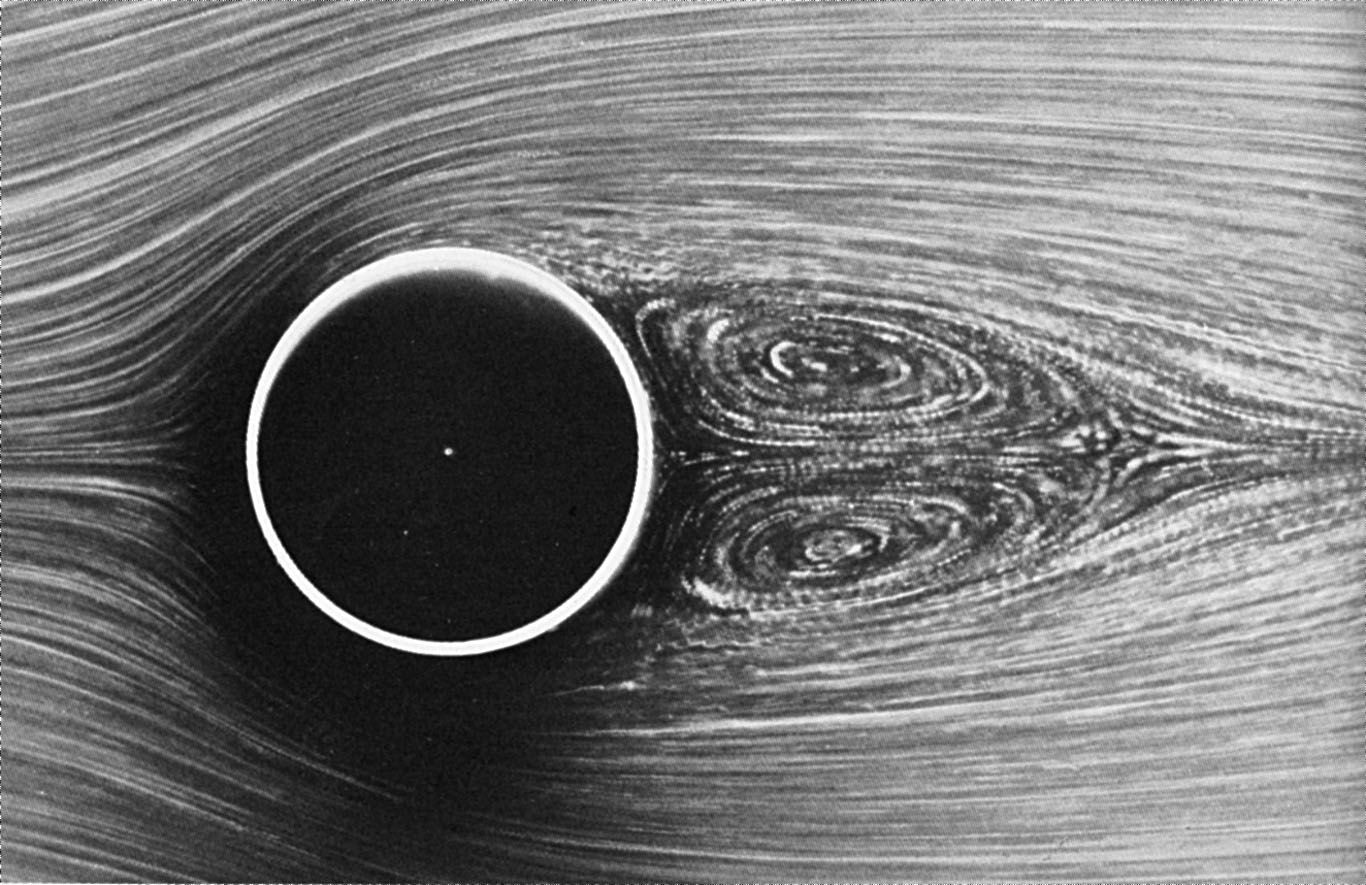
\includegraphics[width=0.95\linewidth]{gd_cylinder.png}
    \captionof{figure}{Обтекание цилиндра}
    \label{fig:cylinder}
\end{minipage}
%
\begin{minipage}[t]{.5\textwidth}
    \centering
    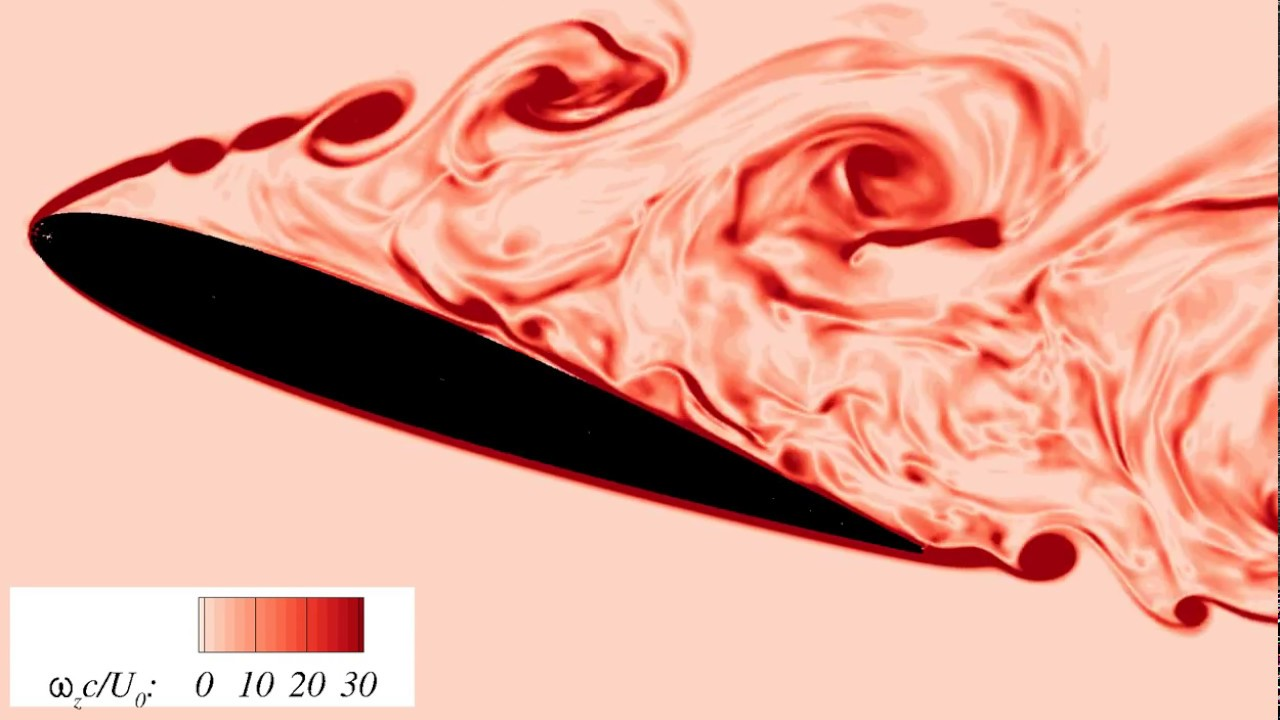
\includegraphics[width=0.95\linewidth]{airfoil.png}
    \captionof{figure}{Обтекание профиля крыла}
    \label{fig:airfoil}
\end{minipage}
\end{verbatim}
}

Если нужно, чтобы рисунки имели общую подпись и собственное буквенное обозначение, то это можно сделать так:

{\small
\begin{verbatim}
\begin{figure}
    \centering
    \begin{subfigure}[b]{0.5\textwidth}
        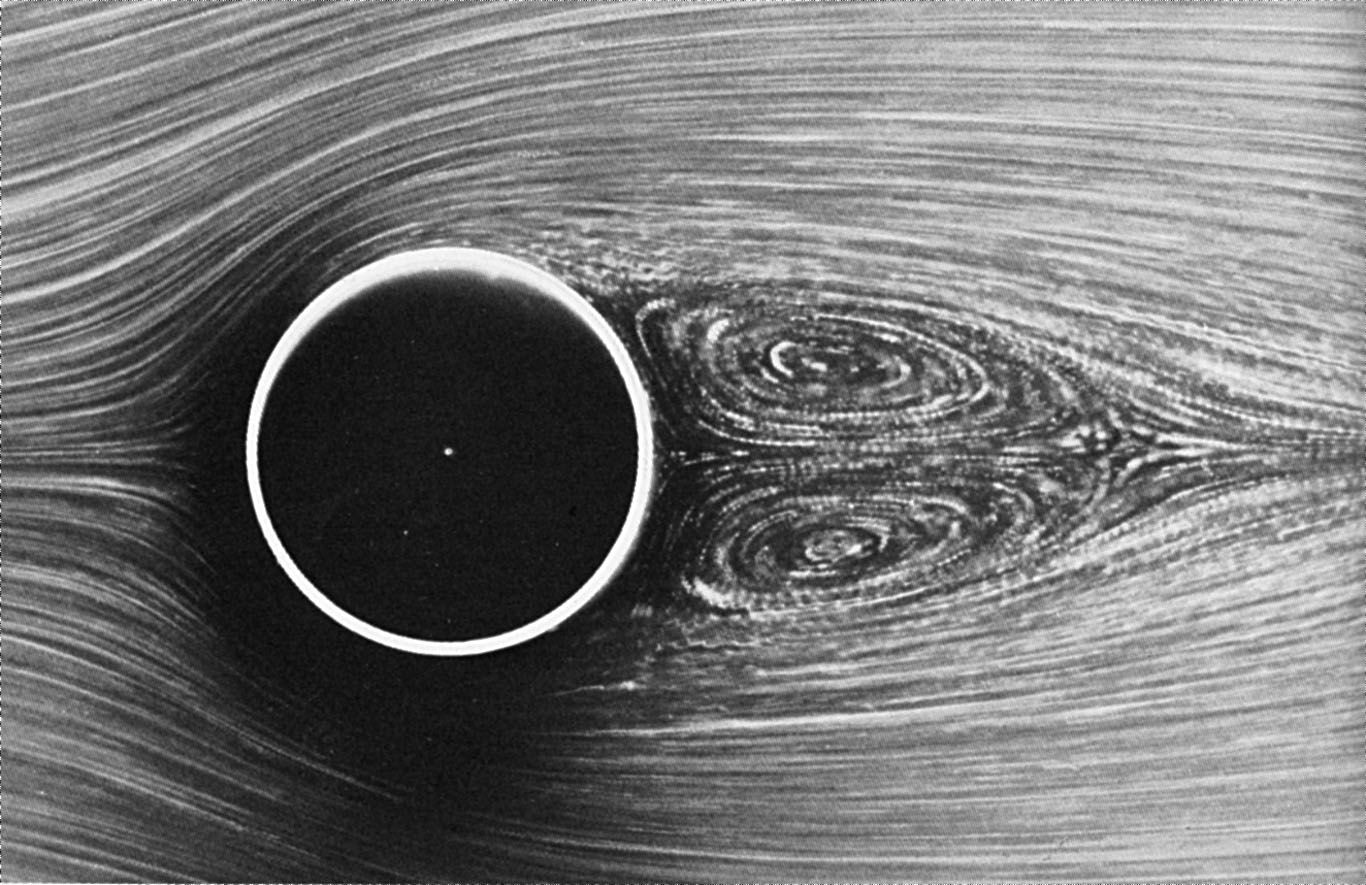
\includegraphics[width=0.95\textwidth]{gd_cylinder.png}
        \caption{цилиндр}
        \label{fig:a_cylinder}
    \end{subfigure}%
    \begin{subfigure}[b]{0.5\textwidth}
        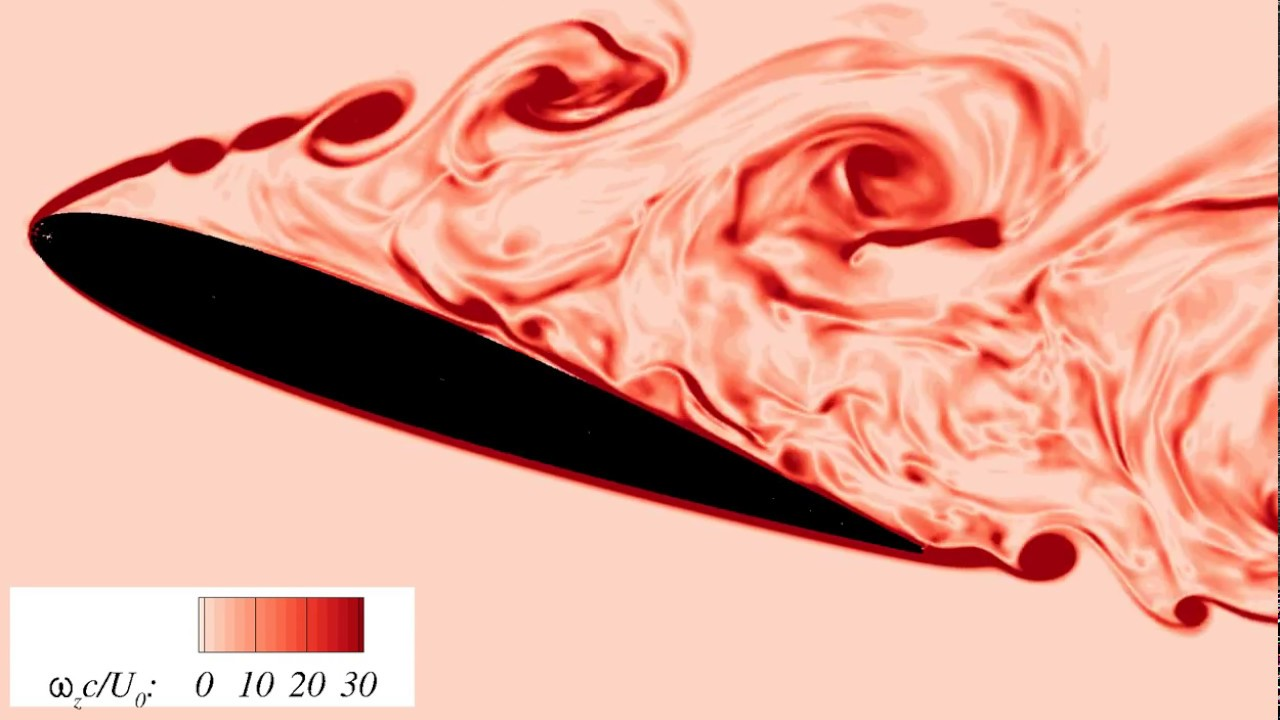
\includegraphics[width=0.95\textwidth]{airfoil.png}
        \caption{профиль крыла}
        \label{fig:subfigure2}
    \end{subfigure}
    \caption{Обтекание различных тел}
    \label{fig:aerodynamics}
\end{figure}
\end{verbatim}
}

\noindent
Это даёт рис.~\ref{fig:aerodynamics}.

\figspace
\begin{figure}[h]
    \centering
    \begin{subfigure}[b]{0.5\textwidth}
        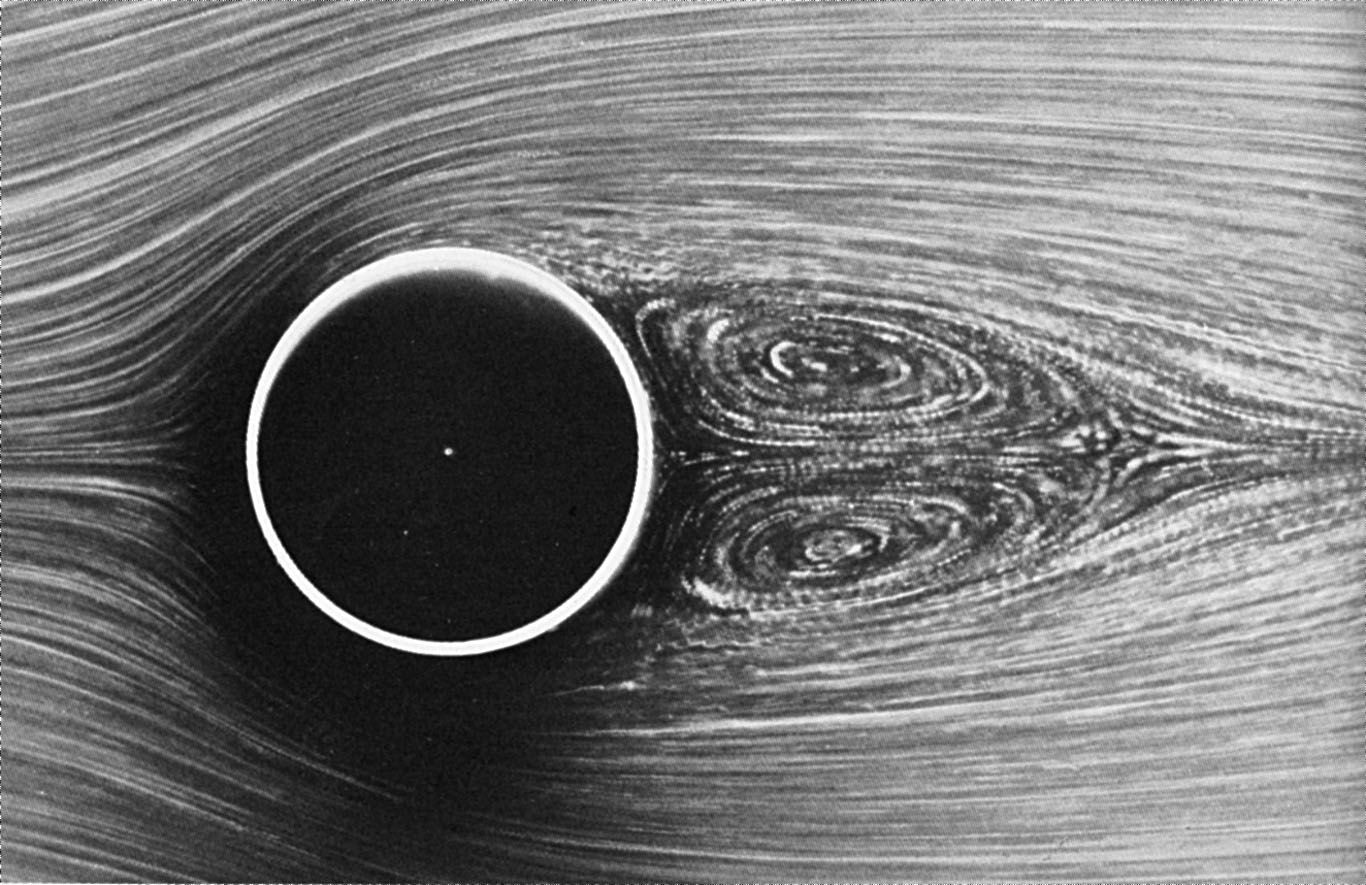
\includegraphics[width=0.95\textwidth]{gd_cylinder.png}
        \caption{цилиндр}
        \label{fig:a_cylinder}
    \end{subfigure}%
    \begin{subfigure}[b]{0.5\textwidth}
        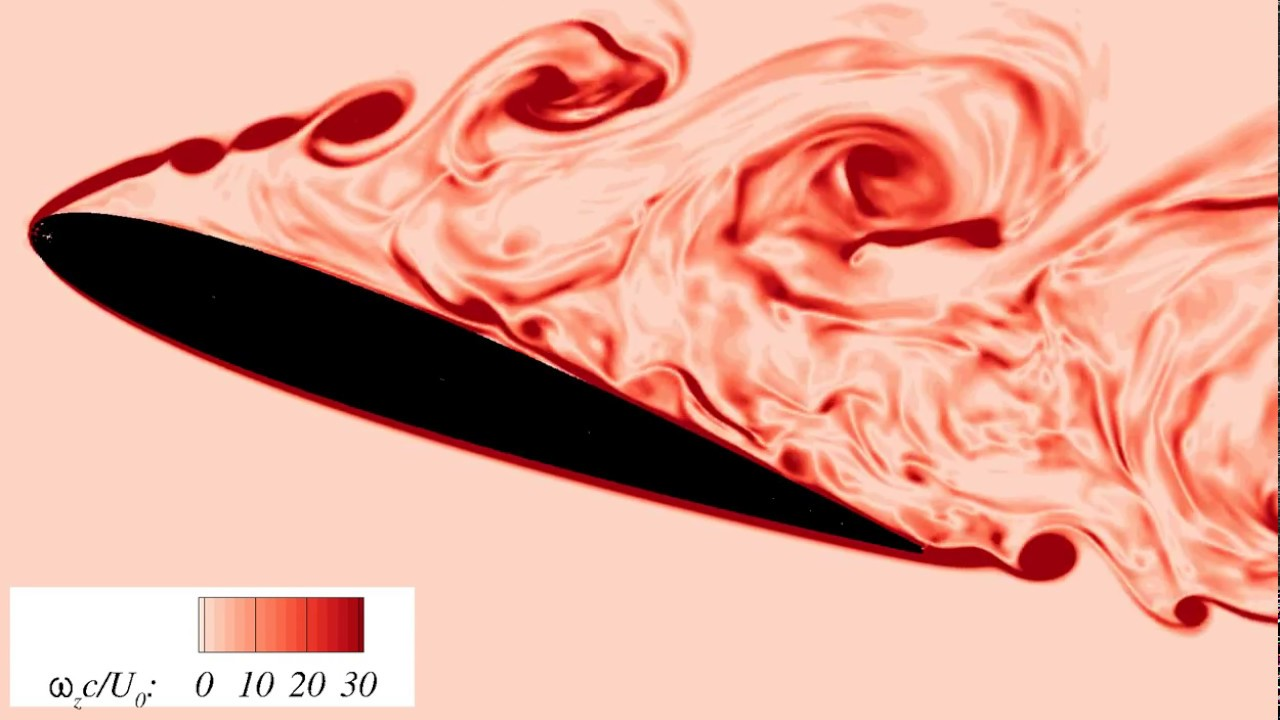
\includegraphics[width=0.95\textwidth]{airfoil.png}
        \caption{профиль крыла}
        \label{fig:subfigure2}
    \end{subfigure}
    \caption{Обтекание различных тел}
    \label{fig:aerodynamics}
\end{figure}
\figspace

\end{document}
